% language syntax and the compiler, the notions of locality and parallelism and how they are orthogonal
% concepts in Chapel

\section{Chapel base language}
\chapter{Chapel base language}
\subsection{} % creates page markers at the top

\begin{frame}{Why another language?}{\url{http://chapel.cray.com}}
  \begin{itemize}\setlength{\itemsep}{1mm}
    \item Shared- and distributed-memory parallelism intrinsic part of the language
    \item Much higher-level (and much easier to use!) than MPI
    \medskip
    \begin{itemize}\setlength{\itemsep}{1mm}
      \item ``Python for parallel programming''
      \item few lines of Chapel code typically replace $\sim$100 lines of MPI code
    \end{itemize}    
    \item Focus on performance
    \medskip
    \begin{itemize}\setlength{\itemsep}{1mm}
      \item simple Chapel codes perform as well as optimized C/C++/F90 code
      \item very complex Chapel codes run at $\sim$70\% performance of a similar well-tuned MPI code (not
      bad in my opinion, but room to improve)
    \end{itemize}    
    \item Perfect language for learning parallel programming for beginners
    \item Open-source: can compile on all Unix-type platforms, precompiled for MacOS
    \item Chicken-and-egg situation: too few people know/use Chapel ~$\Longleftrightarrow$~ too few HPC
    centers install and promote it
  \end{itemize}
\end{frame}

\begin{frame}{Brief history}
\end{frame}

\begin{frame}{Useful links}
  \begin{itemize}\setlength{\itemsep}{3mm}
    \item Getting started guide for Python programmers
    {\small\url{http://chapel-for-python-programmers.readthedocs.io/basics.html}}
    \item Data parallelism in Chapel \url{http://chapel.cray.com/tutorials/ACCU2017/03-DataPar.pdf}
    \item Short tutorial from David Bunde \url{http://faculty.knox.edu/dbunde/teaching/chapel}
    \item docs and examples for various Chapel modules in \texttt{\$CHPL\_HOME/modules/}, e.g.,
    \texttt{standard/} or \texttt{dists/}
    \item \url{https://learnxinyminutes.com/docs/chapel}
    \item \url{https://stackoverflow.com/questions/tagged/chapel}
  \end{itemize}
\end{frame}

\begin{frame}{Exercise: using functions and control flow}
  Write a Chapel code to find the root of the equation $x^5 + 8x^3 - 2x^2 + 5x - 1.2 = 0$ using the bisection
  method in the interval [-1,1]
  \begin{columns}[]
    \column{0.45\textwidth}
    \begin{itemize}\setlength{\itemsep}{3mm}
      \item Calculate the function at the ends and the midpoint of the interval
      \item Depending on the signs of the three computed values, let the midpoint be either the new left
      or the new right end
      \item Repeat until your error is below $\Delta x=10^{-8}$
    \end{itemize}
    \column{0.55\textwidth}
    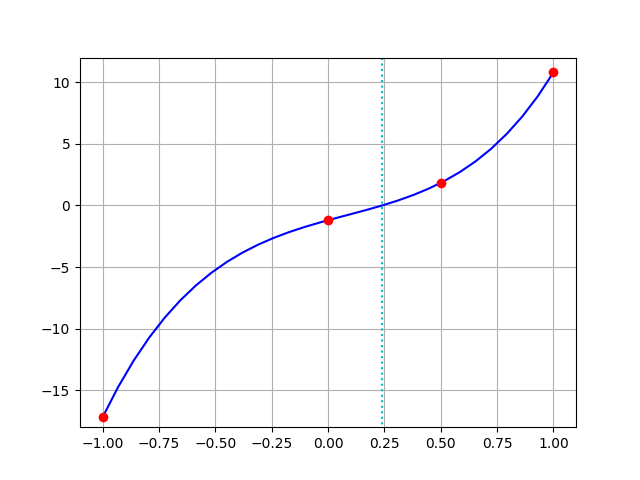
\includegraphics[width=0.95\columnwidth]{figs/bisection.png}
  \end{columns}
\end{frame}
